\section{The political landscape: Theory and empirics}
A Principal Component Analysis (PCA) is a multivariate analysis method within unsupervised statistical learning for reducing dimensions in a parameter space. Our VAA-data is really a 15-dimensional parameter space, making it impossible to visualize all dimensions in a meaningful way. By using PCA we can retain as many dimensions as we wish, but by plotting the two dimensions that explain the most variance in the data we can construct a meaningful static visualization. 
We use the princomp to do our PCA, which progresses in several stages - firstly, a correlation matrix $\sigma$ of the data matrix $X$ is constructed. For each eigenvector $\alpha$, corresponding to this correlation matrix, we want to find the eigenvectors that maximize the variance of the data, i.e. $\alpha’\sigma\alpha$. This can be seen as a Lagrange optimization, subject to $\alpha’\alpha=1$ due to normalization. 
\begin{center}
$\alpha’\sigma\alpha-\lambda( \alpha’\alpha-1)$, differentiation wrs. $\alpha_i$ gives $\sigma\alpha_i-\lambda\alpha_i$
\end{center}

Hence, $\lambda$ can be seen as an eigenvalue to $\sigma$ and $\alpha_i$ is the corresponding eigenvector. The (in our case 15) eigenvectors, called “loadings” in princomp, are then constructed so that the corresponding eigenvalues are maximized and in decreasing order throughout the components. Lastly the “scores” are computed by multiplying the original, standardized values from $X$ with our loadings. This provides us with transformed variable values for each component suitable for plotting. Thus, the “loadings” can be seen as a measure of “importance” from the different parameters - i.e. which questions provide the most explanatory power?
By summarizing our princomp analysis we see that the first component explain 54\% of the variance in the entire data matrix. The second component explains 12\% which gives us a cumulative proportion of 66\% when plotting the first two components.
\begin{figure}[H]
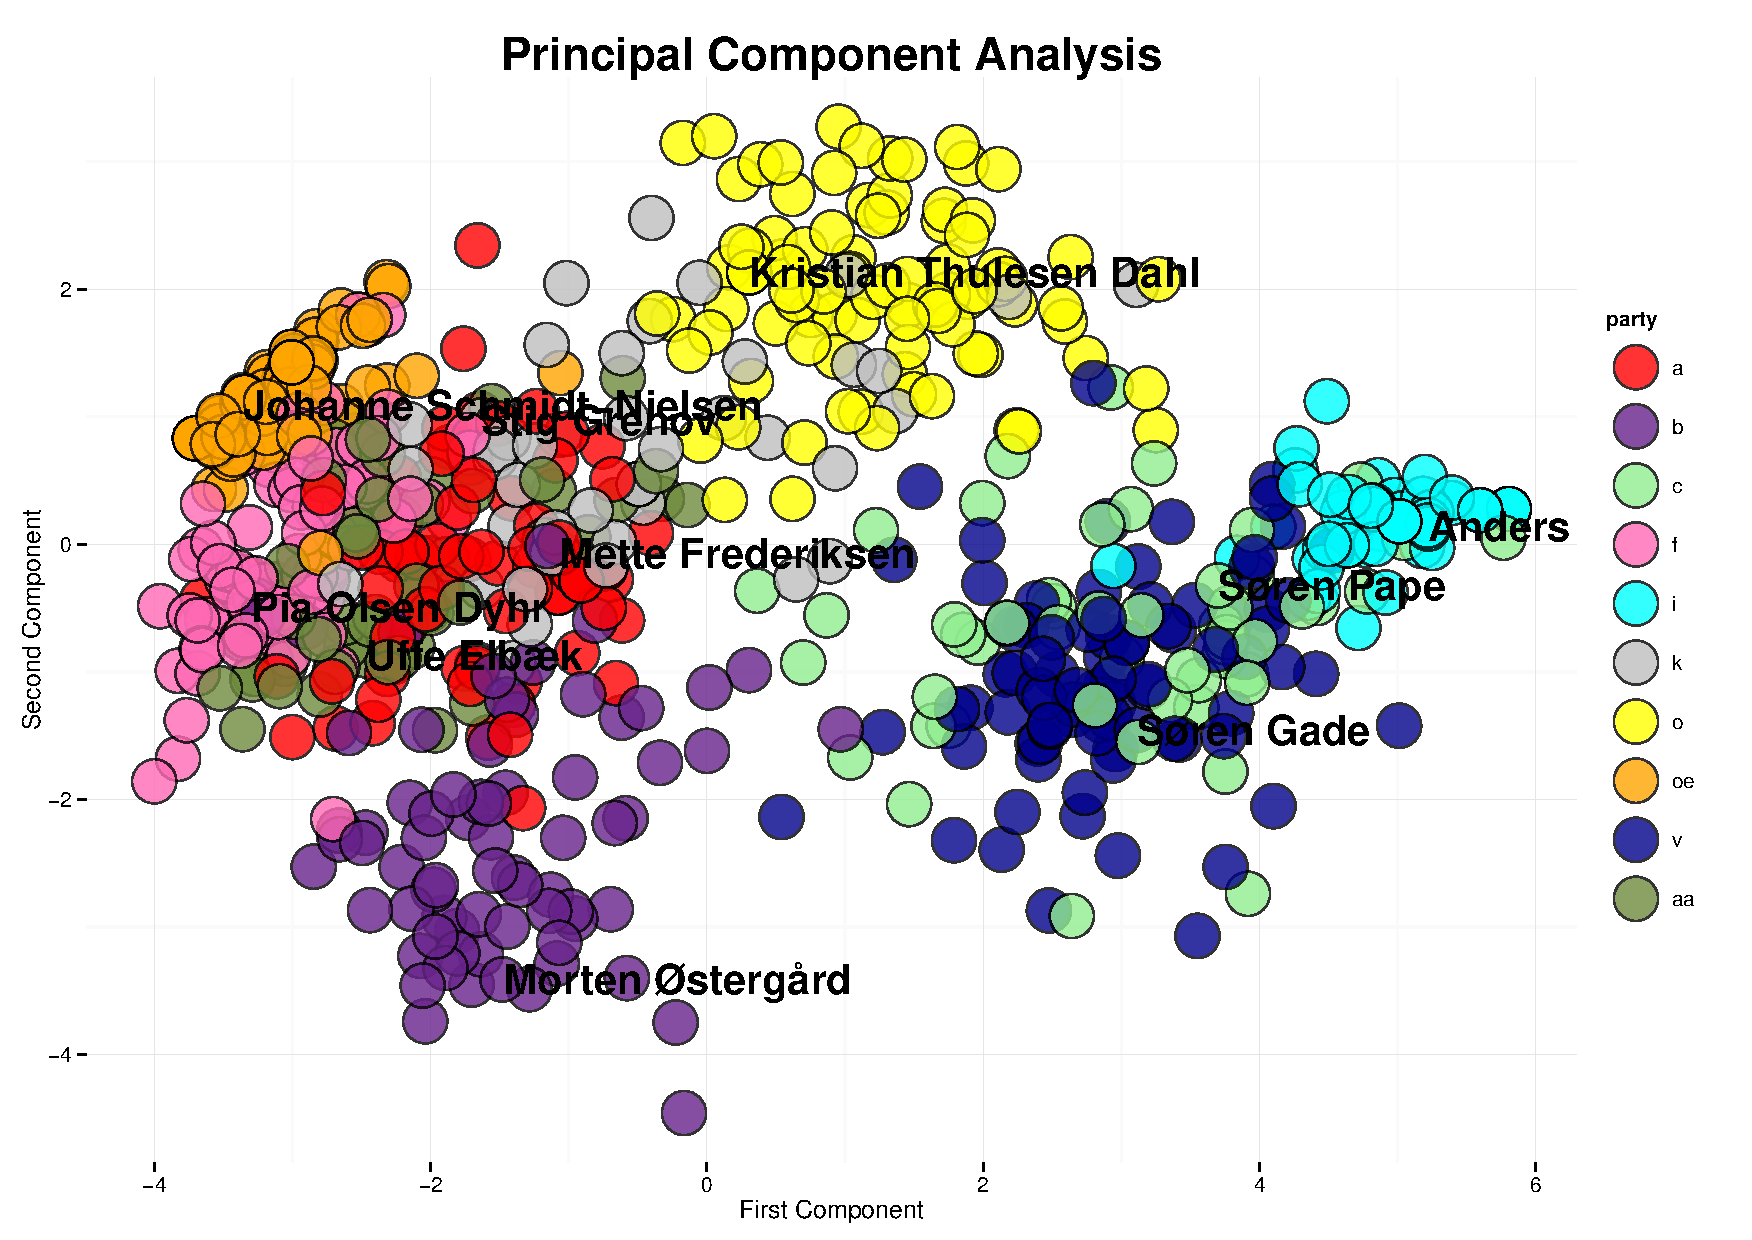
\includegraphics[width=\textwidth]{PCA1}
\end{figure}
The first thing we notice from the PCA plot is that there seems to be a nice grouping of the parties and that a classical left-right scale seems to appear on the horizontal axis (first component). The left wing parties seem to group together to the left, with Enhedslisten clustered together and Socialdemokratiet and Alternativet slightly more spread out. To the right the candidates from Liberal Alliance is also clustered neatly together whereas both Venstre and Konservative are vastly spread out. It is also visually clear that the first component contains the most variance since the vertical axis (second component) mainly contributes with the information that Radikale Venstre and Dansk Folkeparti seemingly are opposed to each other in this dimension. 
As mentioned it seems that the first component, portrayed as the horizontal axis, could be capturing the classical left/right-socialism/liberalism spectrum, driven by distributional politics. Political theory would predict the secondary axis to be driven by value-based politics which makes sense having Radikale and DF opposed to each other - but this does not also explain Enhedslisten and DF supposedly sharing the same values. In fact it seems that the parties that are sharing the same values on the vertical scale usually agree on matters of EU. Let us take a look at the loadings for the first two components to see which variables (questions) are driving  the distribution of the parties in the spectrum plot.
\begin{figure}[H]
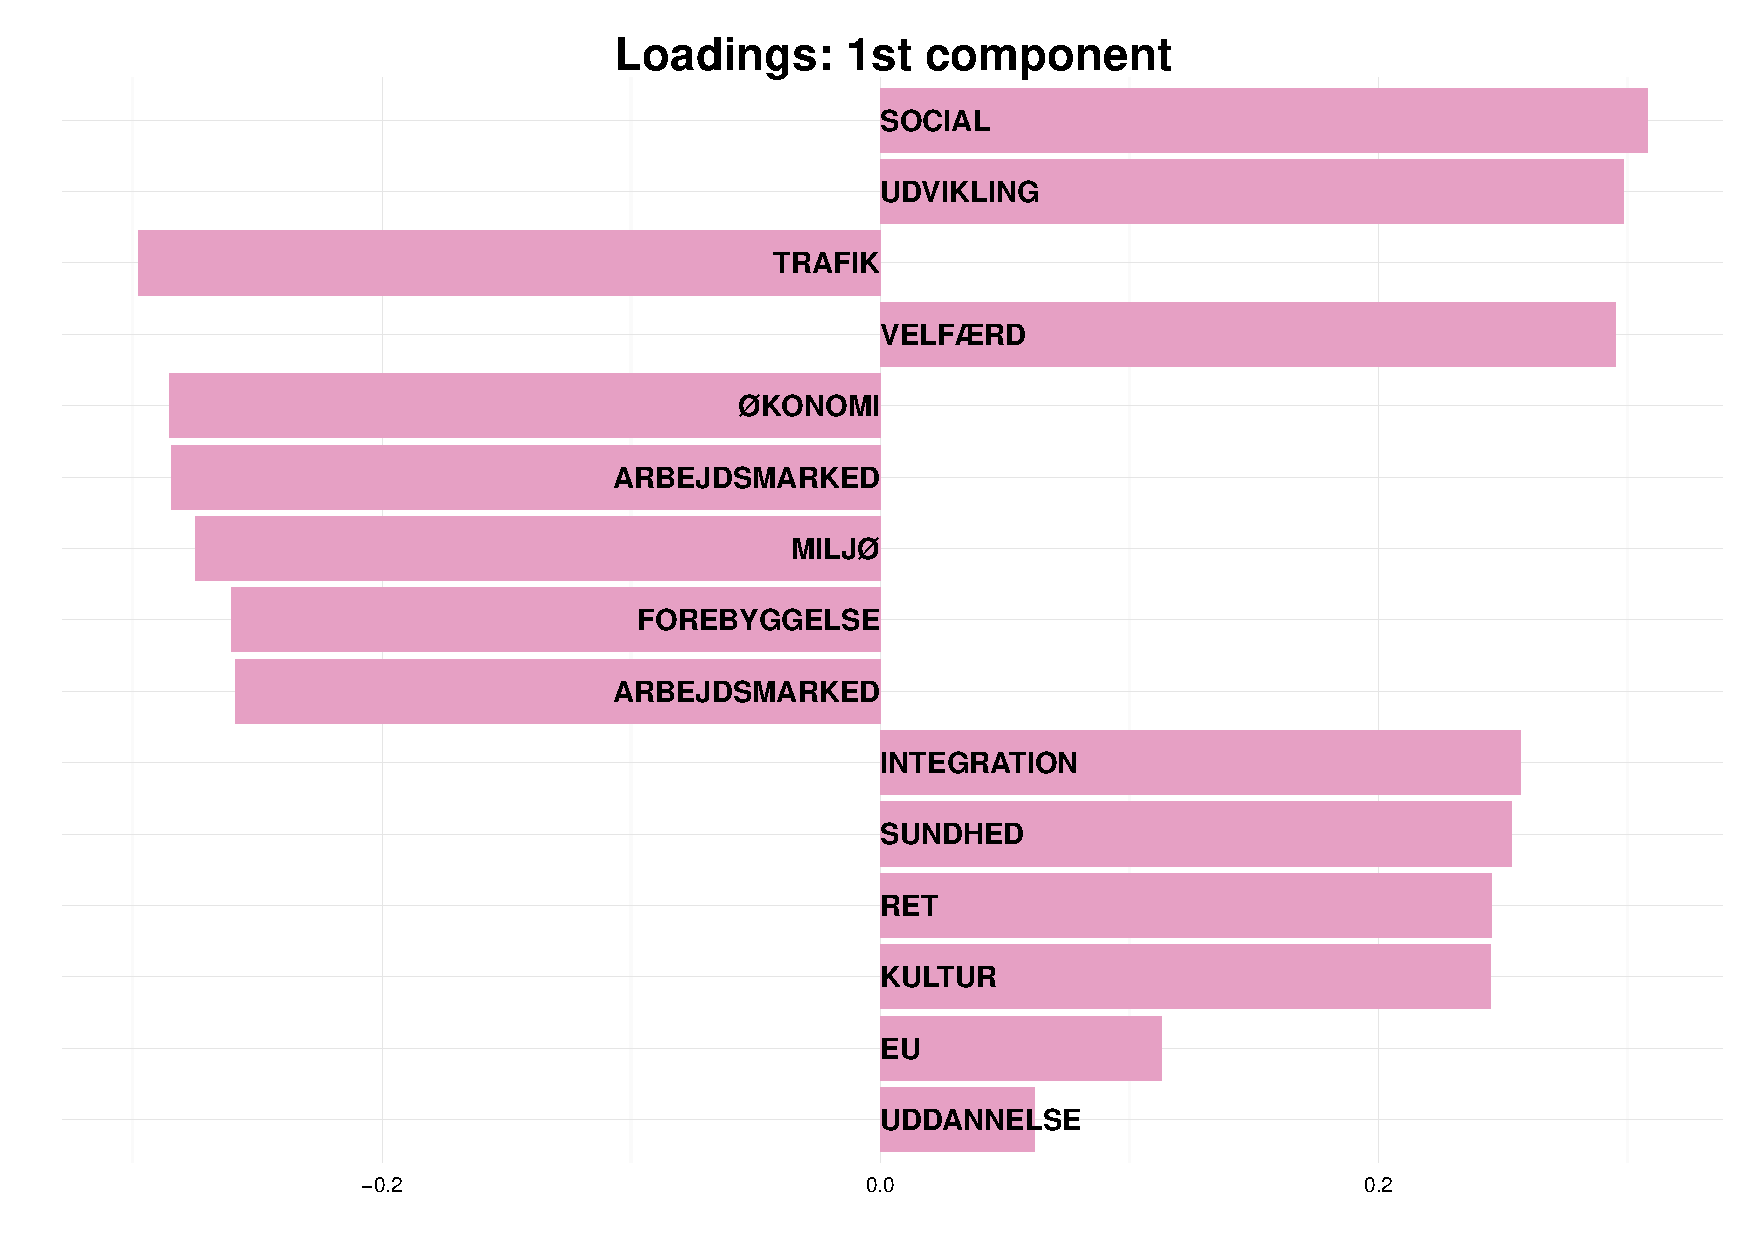
\includegraphics[width=0.5\textwidth]{loadings1}
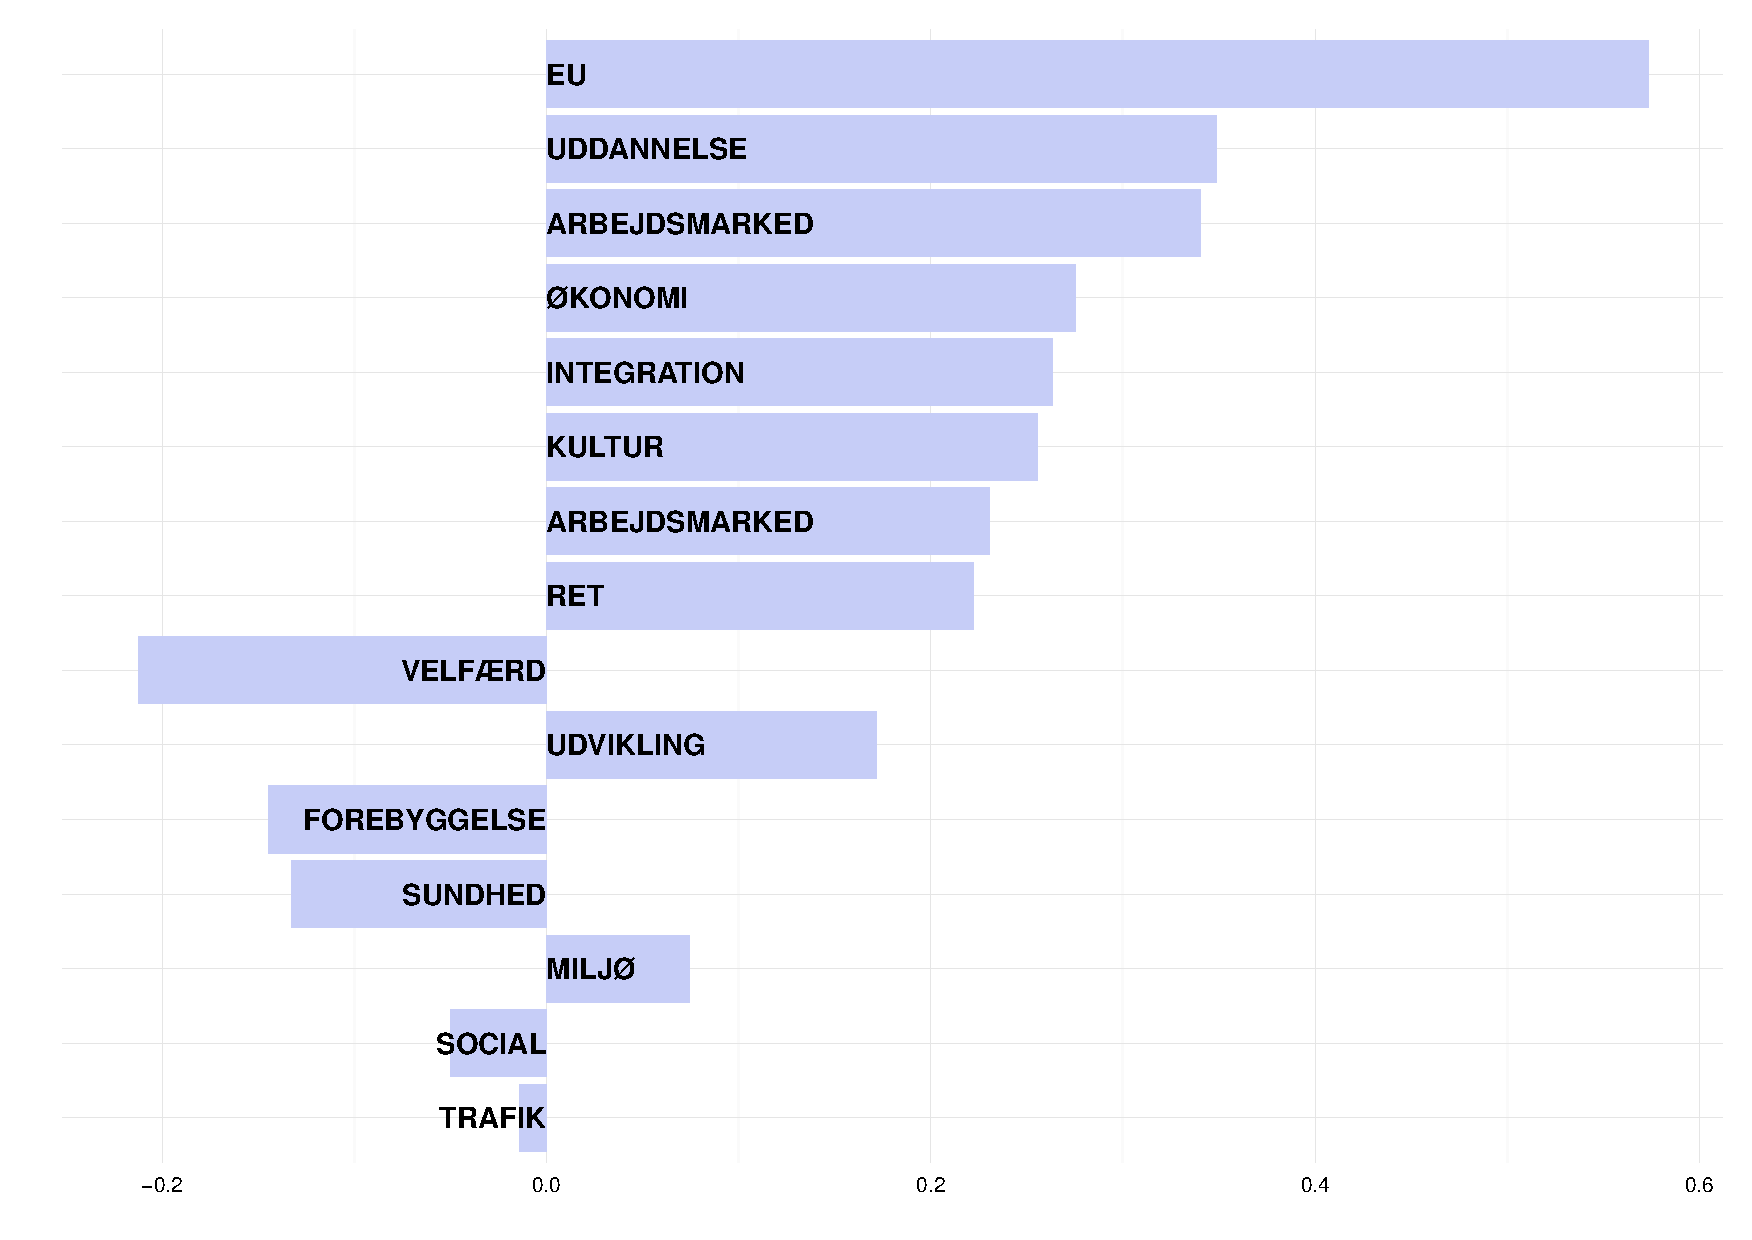
\includegraphics[width=0.5\textwidth]{loadings2}
\end{figure}
The two plots depict the loadings of the first two component in the PCA, ordered according to the loadings’ absolute value. As we see from the left figure, the variation in the first component is mainly driven by questions on welfare benefits, development aid and investments in public transport. As anticipated the loadings of the second component is driven mainly by the question on EU’s role and influence, but also by questions on the public school reform and unemployment benefits. 
A reason why we may not see a crystal clear political spectrum aligned with the political science literature could also be the weighting of the different questions - or rather, the lack thereof. One could argue that a candidate’s views on criminal justice and integration should not weigh as heavily as views on public sector size and levels of unemployment benefits when trying to depict the candidates on a distributional left-right-scale. Vice versa we would want issues on integration and environmental politics to weigh more when plotting the value-based political spectrum. The candidates are not asked to weigh the questions individually (as seen in FINNISH paper, ref.)
Therefore we try and subset our initial dataset into two separate datasets grouped by questions regarding distributional and value-based politics respectively. Questions on distributional politics are statements such as “Growth in the public sector is more important than tax reliefs”, “Unemployment benefits should be lowered, making it more profitable to take a job” and “A visit to the general practitioner should cost 100DKR.”. Questions on value-based politics are statements like “Public institutions are too considerate towards religious minorities” and “EU have too much power over Danish law”. We perform two separate PCAs on these segregated datasets and plot the two first components in the same plot, in order to see if the political spectrum is more visible now.

[Nyt PCA-plot]

Again, we try to plot the distributional political views on the x-axis and the value-based political views on the y axis. Our new plot differs from the original PCA plot in two ways - the parties are more difficult to entangle and there seems to be a strong correlation between the two axes. 